\documentclass[../main.tex]{subfiles}

\begin{document}

\section{Estructuras sismorresistentes}

\href{https://youtu.be/6VVqDEFBOIk}{Clase 1 (20210420)}

El reglamento pertinente es el Reglamento CIRSOC 103, que tiene tanto comentarios
como sus distintas partes.

Se parte de un mapa desde donde se registra la zonificación sismica argentina, 
desde donde se verá el tipo de actividad esperada. También es importante la
clasificación del suelo sobre el que nos encontramos, por ejemplo con el 
ensayo SPT. Por último, segun el tipo de la construcción y su destino se lo clasifica
entre $A_o$, $A$, $B$, $C$, donde cada uno será afectado con un coeficiente de
seguridad $\gamma$. Todo esto se encuentra en el Cap. 2 del CIRSOC 103.

\subsection{Métodos de evaluación: verificación simplificada}

Definida en 2.7.1. destinada a estructuras de baja altura. Ver. % COMPLETAR
El proceso consiste:

\begin{enumerate}
  \item Encontrar el coeficiente sísmico de diseño como $C=C_n \gamma_r$. Depende
    el $C_n$ de la zona sísmica.
   \item Resultante de las fuerzas horizontales equivalentes o esfuerzo de corte
     en la base de la construcción como $V_o = C*W$.
\end{enumerate}

El valor de $W$ se calcula como  $W=\Sigma W_i$, por lo que dependiendo de la alutra
se tendrán distintos pesos $W$, incrementando la magnitud de las fuerzas 
horizontales.


\subsection{Método estático}

La acción sísmica se considera equivalente a la acción de un sistema de fuerzas,
paralelo a la dirección analizada y aplicada en los centros de las masas que 
conforman el modelo estructural.

Este método esta limitado por lo siguiente:

% Table generated by Excel2LaTeX from sheet 'Hoja1'
\begin{table}[htbp]
  \centering
    \begin{tabular}{|l|r|r|r|}
    \hline
    \multicolumn{1}{|c|}{\multirow{2}[4]{*}{Zona sísmica}} & \multicolumn{3}{c|}{Altura máxima (m)} \bigstrut\\
\cline{2-4}          & \multicolumn{1}{l|}{Ao} & \multicolumn{1}{l|}{A} & \multicolumn{1}{l|}{B} \bigstrut\\
    \hline
    3 y 4 & 12    & 30    & 45 \bigstrut\\
    \hline
    0, 1 y 2 & 16    & 45    & 60 \bigstrut\\
    \hline
    \end{tabular}%
\end{table}%

Luego de verificar esto, se requiere:

\begin{enumerate}
  \item Ubicar la zona sísmica de la estructura.
  \item Adoptar un factor de riesgo.
  \item Evaluar aplicabilidad del método estático
\end{enumerate}

\subsubsection{Aplicabilidad del método estático}

Además del tema de la altura, se deben verificar aspectos tales como:

\begin{description}
  \item[Regularidad en planta] se debe considerar la regularidad torsional,
    continuidad de los elementos resistentes y ortogonalidad o simetría de los
    elementos resistentes.

    Una estructura es irregular cuando la respuesta en cada sentido provoque una
    rotación de la misma, lo que puede crear una concentración de esfuerzos en una
    determinada zona y puede provocar otros problemas.

  \item[Regularidad en altura] se debe tener una regularidad en la rigidez,
    masas, dimensiones horizontales, configuración vertical de los elementos
    resistentes y resistencia lateral.

    Es importante la regularidad de la rigidez, porque se pueden dar ciertos $\Delta$
    en la inclinación de la estructura, y que puede dar problemas en la estabilidad.
    Eso se da, por ejemplo, porque un piso sea mucho más flexible que otro.
\end{description}

Todo esto queda definido en la siguiente tabla:

\begin{figure}[ht]
  \centering
  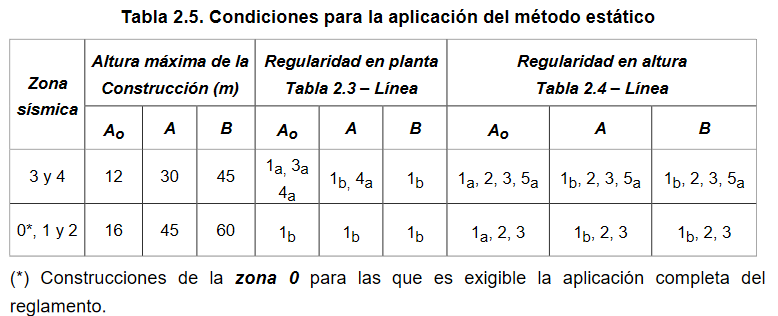
\includegraphics[width=0.8\textwidth]{../images/20210420/tabla1}
\end{figure}


\subsubsection{Espectro sísmico} \label{espect}

Depende de la respuesta temporal de cada estructura, que nos dará un valor
de deformación, velocidad, etc en el tiempo.

\begin{figure}[ht]
  \centering
  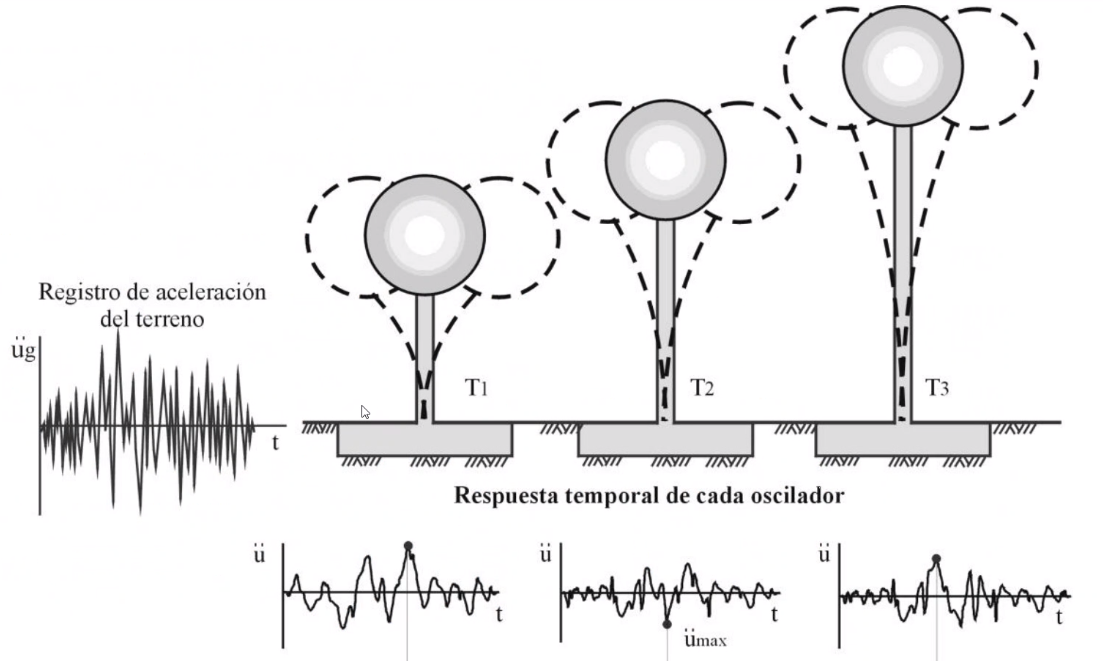
\includegraphics[width=0.8\textwidth]{../images/20210420/espectro}
\end{figure}

Lo que nos importará de este diseño será la máxima amplitud $A$, que en estos
casos se ve delineado con $u_{max}$. La ejecución de uno de estos esquemas es 
muy complicado, por lo que el reglamento permite el uso de $N_{v}=1.2$ y $N_a=1$,
y a partir de la tabla 3.1 nos permite adoptar los valores de $a_{s}$, $C_{a}$
y $C_v$. 

\begin{figure}[ht]
  \centering
  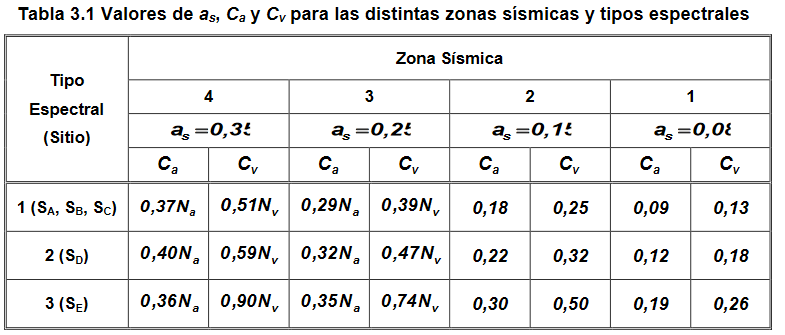
\includegraphics[width=0.8\textwidth]{../images/20210420/3_1}
\end{figure}

Luego, conocidos estos valores podemos obtener el valor de $T_2$ que es el 
período característico del espectro:

\begin{align*}
  T_2 &= \frac{C_v}{2.5*C_a} \\[5pt]
  T_1 &= 0.2 * T_2
.\end{align*}

Por último, según sección 3.5.1. obtenemos el valor de $S_a$, que son las ordenadas
del espectro elástico. Dependerá de $T$, $T_1$ y $T_2$.

\subsubsection{Cálculo de periodo}


Conocido los valores ya vistos en \Cref{espect}, es posible encontrar el valor
de $T$ como:

\begin{align*}
  T = 2*\pi *\sqrt{\frac{\Sigma * W_i u_i^2}{g*\Sigma*F_i*u_i}} 
.\end{align*}

El valor de $u_i$ es el corrimiento para la fuerza  $F_i$.
Donde el valor de $F_i$ es la fuerza sísmica horizontal $F_i$ aplicada en el 
baricentro de la carga gravitatorio como:

 \begin{align*}
  F_i = \frac{W_i*h_i}{\Sigma W_i*h_i}
.\end{align*}

El valor del período obtenido debe verificar la siguiente ecuación:

\begin{align*}
  T &\leq C_u * T_a  \\[5pt]
  T_a &= C_f * H^x
.\end{align*}

Donde el valor de $C_u$ depende del valor de $a_s$ y el valor de  $C_s$ y $x$ salen
de la tabla 6.3 de CIRSOC 103.

\begin{figure}[ht]
  \centering
  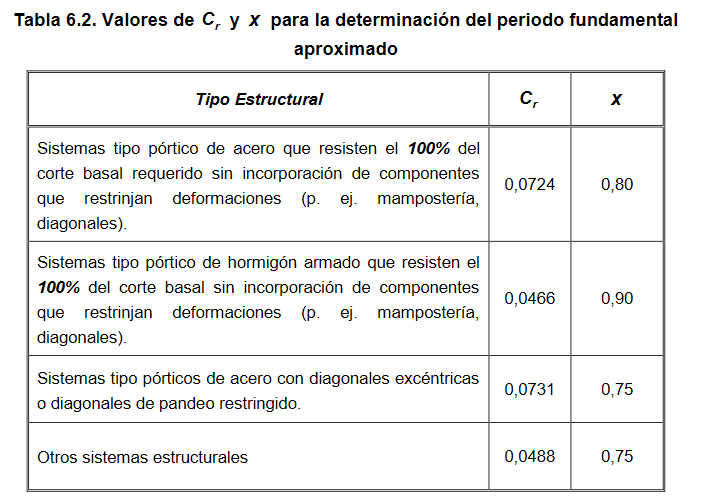
\includegraphics[width=0.8\textwidth]{../images/20210420/tabla6_3}
\end{figure}

\subsubsection{Establecer factor de reducción último R}

Según el tipo de estructura, se debe definir el factor de reducción por comportamiento
último $R$ como:

 \begin{align*}
   R = \frac{V_E}{V_s}
.\end{align*}

Este valor se ve relacionado con la ductilidad de la estructura.

\subsubsection{Formula base}

Conociendo la zona sísmica y el factor de riesgo, se puede obtener el valor
del corte basal de la siguiente forma:

\begin{align*}
  V_o &= C*W \tag{Corte en base} \\[5pt]
  W &= \Sigma W_i
.\end{align*}

Donde $W$ es el peso de la estructura, y  $C$ un coeficiente sísmico de diseño,
que se obtiene de las expresiones del CIRSOC 103 en el apartado 6.2.2 en función
del período fundamental de la estructura:

\begin{align*}
  C &= 2.5 C_a \gamma_r / R \hspace{0.25cm} &\xrightarrow{\hspace*{0.5cm}} \hspace{0.1cm}\text{para } T\leq T_2 \\[5pt]
  C &= S_a \gamma / R \hspace{0.25cm} &\xrightarrow{\hspace*{0.5cm}} \hspace{0.1cm} \text{para } T \geq T_2 \\[5pt] 
  C &\geq 0.8 * a_s * N_v / R \hspace{0.25cm} &\xrightarrow{\hspace*{0.5cm}} \hspace{0.1cm} \text{para zona 3 y 4}   \\[5pt]
  C &\geq  0.11 C_a * \gamma_r \hspace{0.25cm} &\xrightarrow{\hspace*{0.5cm}} \hspace{0.1cm} \text{para zonas 0, 1 y 2} 
.\end{align*}


\subsubsection{Fuerzas laterales}

Por último, teniendo todo lo anterior, es necesario adoptar sobrecargas por piso
según reglamento CIRSOC 101, obtener la carga gravitatorio por piso y total $W$ 
de la siguiente forma:

 \begin{align*}
  W_i = D_i + \Sigma f_i * L_l + f_2 * S_i 
.\end{align*}

Y podemos obtener la fuerza basal como:

\begin{align*}
  F_k = \frac{W_k*h_k*V_c}{\Sigma W_i*h_i}
.\end{align*}

\subsubsection{Verificación de esfuerzos torsionales}

% COMPLETAR

\subsubsection{Combinación de acciones ELU}

Debemos considerar esto de la siguiente forma:

% COMPLETAR

\subsubsection{Verificar deformaciones}

Se hace según sección 6.4 y 8.4.
Es necesario verificar las hipótesis de diafragma rígido.


\end{document}
